%% gene_prediction.tex
%% Author: Leighton Pritchard
%% Copyright: James Hutton Institute
%% A brief description of gene prediction, as an illustrative example

% SUBSECTION: Prokaryotic CDS prediction
\subsection{Prokaryotic CDS Prediction}

% Prokaryotic gene prediction
\begin{frame}
  \frametitle{Prokaryotic CDS Prediction Methods}
  Using CDS prediction as an illustrative example for all feature prediction.\\[0.2cm]
  \begin{itemize}
    \item Prokaryotes ``easier'' than eukaryotes for gene/CDS prediction
    \item Less uncertainty in predictions (isoforms, gene structure)
    \begin{itemize}
      \item Very gene-dense (over 90\% of chromosome is coding sequence)
      \item No intron-exon structure
      \item Problem is: ``which possible ORF contains the true gene, and which start site is correct?''
      \item Still not a solved problem
    \end{itemize}       
  \end{itemize}
\end{frame}

% Finding ORFs
\begin{frame}
  \frametitle{Finding Open Reading Frames}
  The simplest approach: find ORFs (sequence between two consecutive in-frame stop codons)
  \begin{itemize}
    \item<1-> ORF finding is naive, does not consider:
    \begin{itemize}
      \item Start codon
      \item Promoter/RBS motifs
      \item Wider context (e.g. overlapping genes)
    \end{itemize}
  \end{itemize}
  Dedicated tools, e.g. \texttt{Glimmer}, \texttt{Prodigal}, \texttt{RAST} usually better.
\end{frame}

% Two alternative methods
\begin{frame}
  \frametitle{Two \textit{ab initio} Prokaryotic Prediction Tools}
  \begin{itemize}
    \item \texttt{Glimmer}\footnote{\tiny{\href{http://dx.doi.org/10.1093/bioinformatics/btm009}{Delcher \textit{et al}. (2007) \textit{Bioinformatics} \textbf{23}:673-679 doi:10.1093/bioinformatics/btm009}}}
    \begin{itemize}
      \item Interpolated Markov models
      \item Can be trained on ``gold standard'' datasets
    \end{itemize}
    \item \texttt{Prodigal}\footnote{\tiny{\href{http://dx.doi.org/10.1186/1471-2105-11-119}{Hyatt \textit{et al}. (2010) \textit{BMC Bioinf.} \textbf{11}:119 doi:10.1186/1471-2105-11-119}}}
    \begin{itemize}
      \item Log-likelihood model based on GC frame plots, followed by dynamic programming
      \item Can be trained on ``gold standard'' datasets
    \end{itemize}
  \end{itemize}
  Applying these to an example bacterial chromosome$\ldots$
\end{frame}

\begin{frame}
  \frametitle{Comparing predictions in Artemis\footnote{\tiny{\href{http://dx.doi.org/10.1093/bioinformatics/btr703}{Carver \textit{et al}. (2012) \textit{Bioinformatics} \textbf{28}:464-469 doi:10.1093/bioinformatics/btr703}}}}
  Not every ORF (green) is predicted to encode for a coding sequence (CDS; blue/orange).\\
  Self-contradictory CDS calls (orange); even automated annotation needs manual curation.
  \begin{center}
    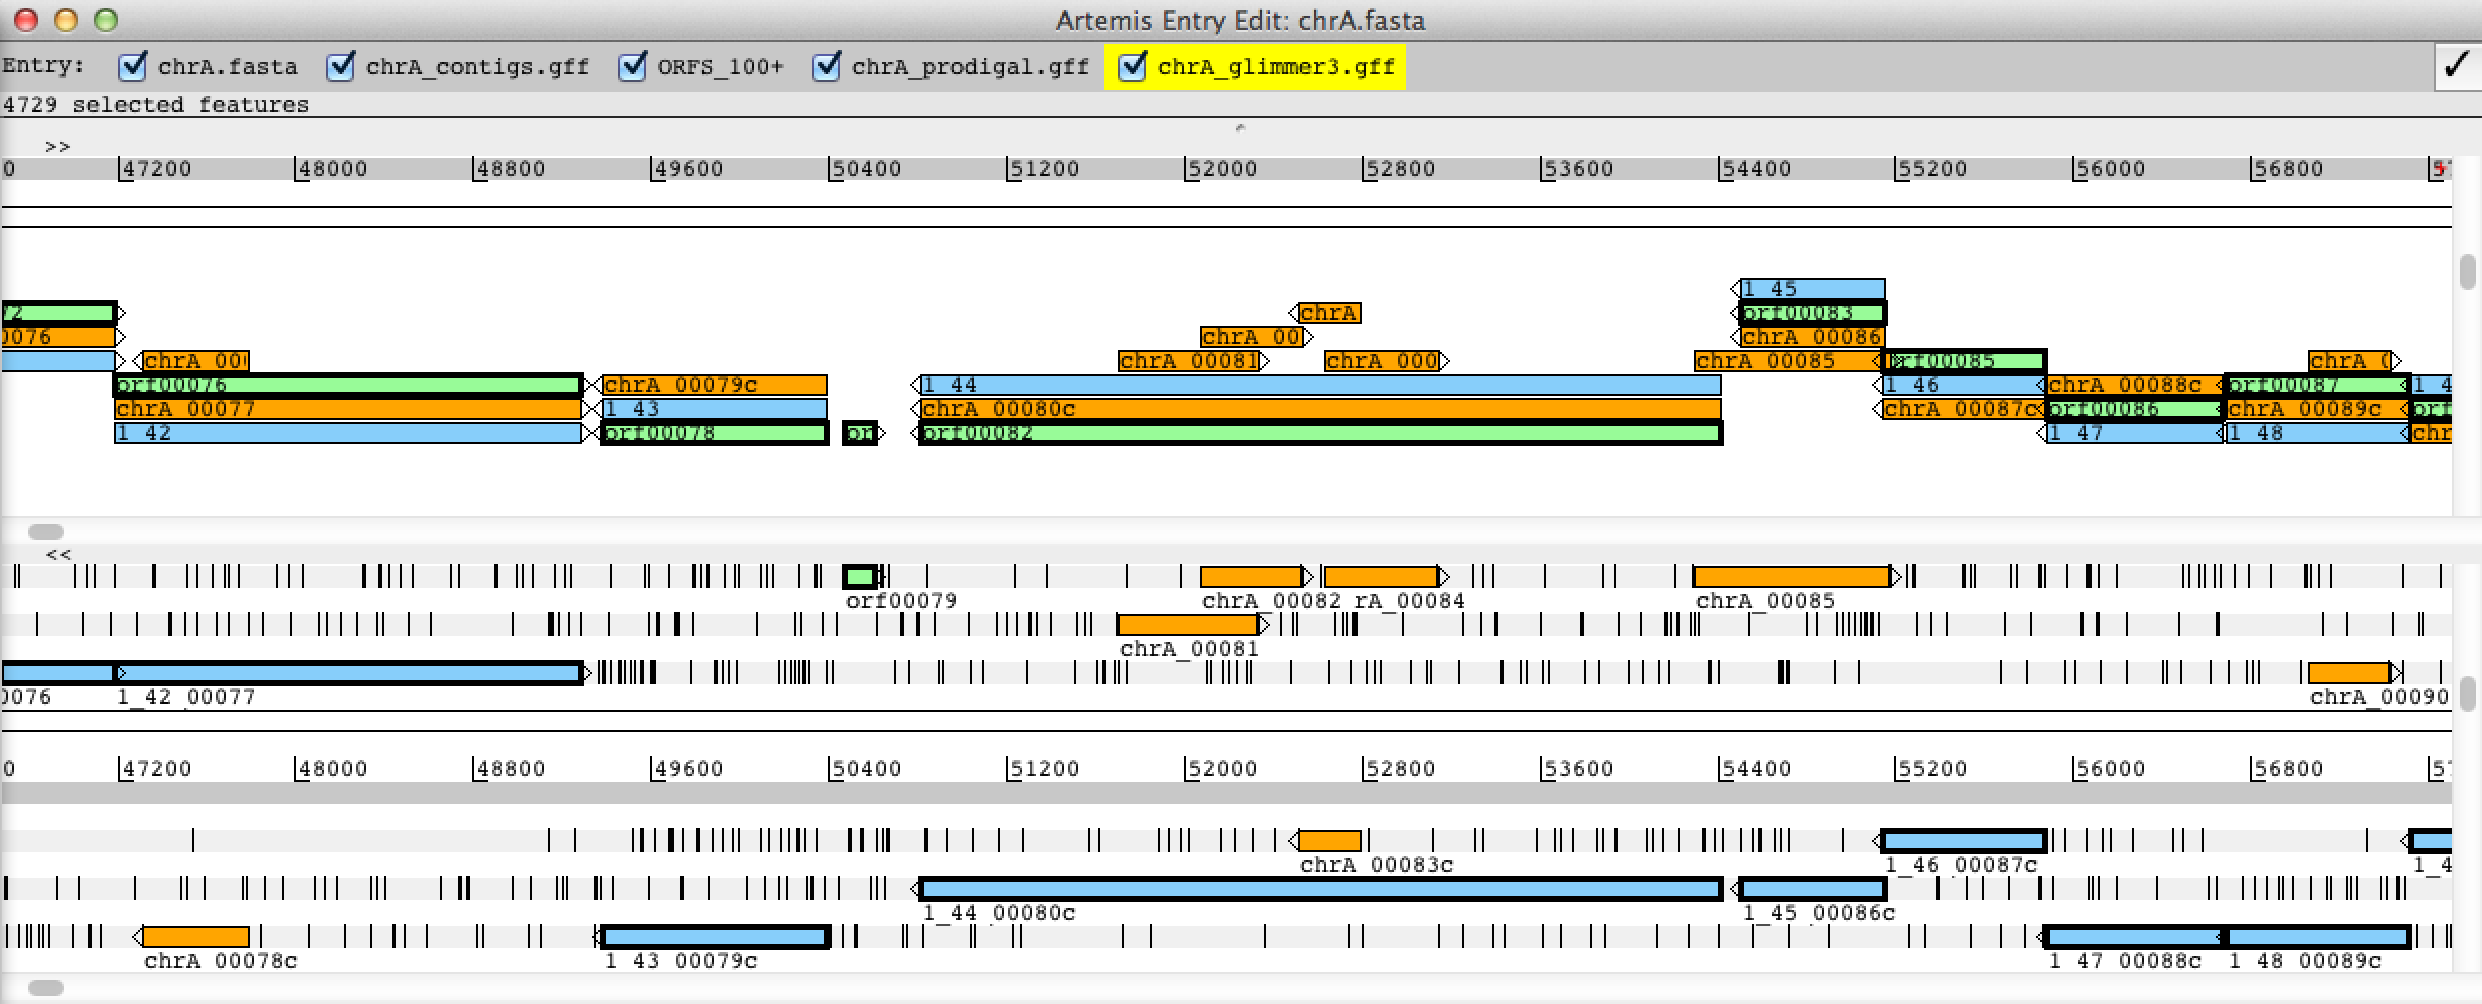
\includegraphics[width=1\textwidth]{images/artemis_cdspred3}     
  \end{center}
\end{frame}

\begin{frame}
  \frametitle{Comparing predictions in Artemis}
  \texttt{Glimmer}(green)/\texttt{Prodigal}(blue) CDS prediction methods do not always agree.
  \begin{center}
    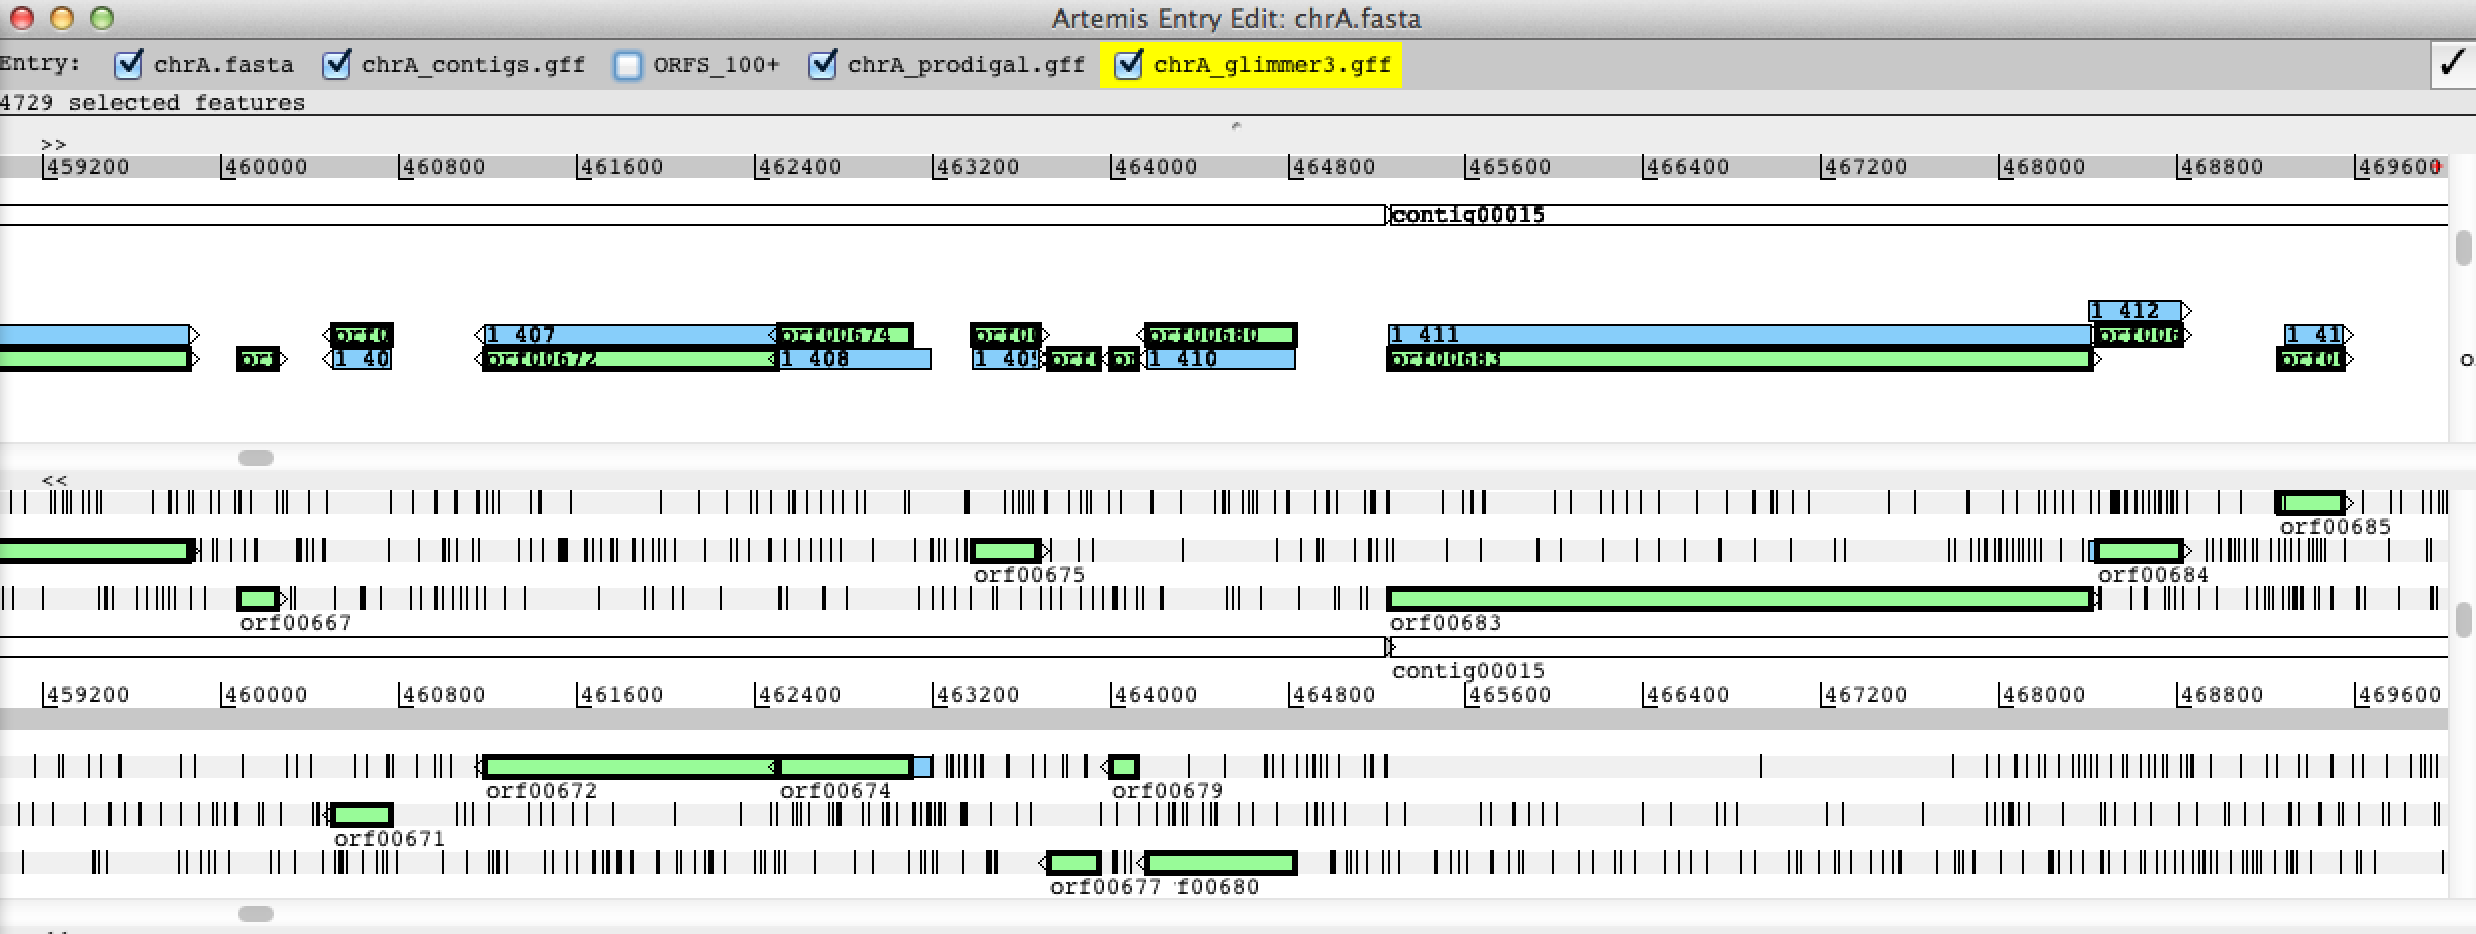
\includegraphics[width=1\textwidth]{images/artemis_cdspred4}     
  \end{center}
  How do we know which (if either) is best?
\end{frame}